\documentclass{article}

\usepackage{graphicx}
\usepackage{tikz}
\usepackage{tikzsymbols}
\usetikzlibrary{calc,patterns,shapes.geometric}
\pagestyle{empty}
\usepackage[margin=0pt]{geometry}
\geometry{papersize={14in,12in}}

\def\centerarc[#1](#2)(#3:#4:#5){\draw[#1] ($(#2)+({#5*cos(#3)},{#5*sin(#3)})$) arc (#3:#4:#5);}

\begin{document}
	\begin{figure}
		\centering
		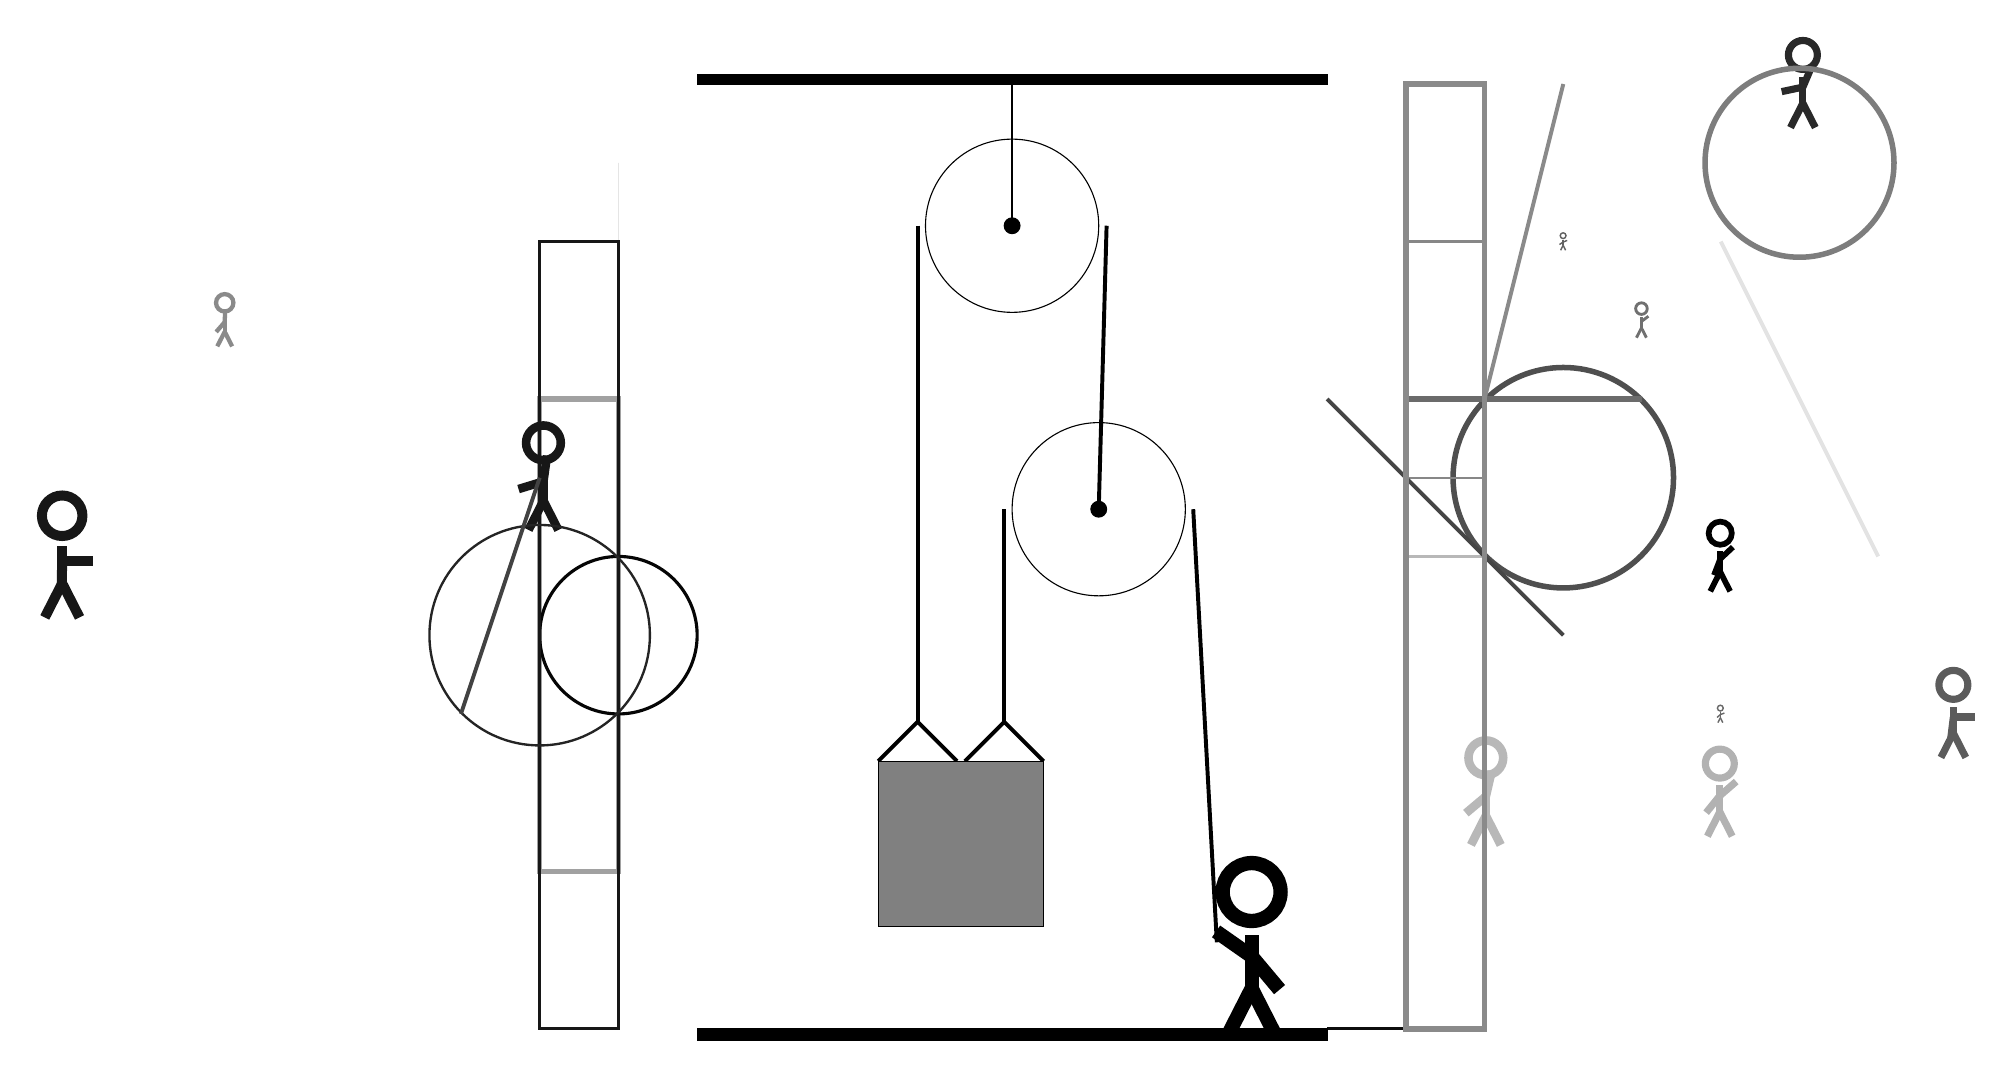
\begin{tikzpicture}
			%%%%% START %%%%%
			
			\draw[fill=black] (-2, 9) rectangle (6, 9.125);
			
			\draw (2, 7.2) circle (1.1);
			\draw[fill=black] (2, 7.2) circle (0.1);
			\draw[thick] (2, 7.2) -- (2, 9);
			
			\draw (3.1, 3.6) circle (1.1);
			\draw[fill=black] (3.1, 3.6) circle (0.1);
			
			\draw[line width = 0.5mm]  (0.3, 0.4) -- (0.8, 0.9) -- (1.3, 0.4);
			\draw[line width = 0.5mm]  (1.4, 0.4) -- (1.9, 0.9) -- (2.4, 0.4);
			\draw[fill=black!50] (0.3, 0.4) rectangle (2.4, -1.7);
			
			\draw[line width = 0.5mm] (0.8, 7.2) -- (0.8, 0.9);
			\centerarc[line width = 0.5mm](2, 7.2)(0:180:1.2000000000000002);
			\draw[line width = 0.5mm] (3.2, 7.2) -- (3.1, 3.6);
			\draw[line width = 0.5mm] (1.9, 3.6) -- (1.9, 0.9);
			\centerarc[line width = 0.5mm](3.1, 3.6)(0:180:1.2000000000000002);
			\draw[line width = 0.5mm] (4.3, 3.6) -- (4.6, -1.9);
			
			\draw[line width=0.5mm, color=black!11](11, 7) -- (13, 3);
			
			\node[line width=0.7mm, color=black!59] at (11, 1) {\Strichmaxerl[1][42][20]};
			\draw[line width=0.7mm, color=black!42] (8, -1) rectangle (8, 6);
			\node[line width=0.2mm, color=black!64] at (14, 1) {\Strichmaxerl[5][83][0]};
			\draw[line width=0.7mm, color=black!37] (-3, 5) rectangle (-4, -1);
			
			\draw [line width=0.4mm, color=black!98](-3, 2) circle (1.0);
			\draw [line width=0.7mm, color=black!69](9, 4) circle (1.4);
			\node[line width=0.3mm, color=black!91] at (-10, 3) {\Strichmaxerl[7][89][0]};
			\draw[line width=0.7mm, color=black!28] (7, 1) rectangle (7, 8);
			\node[line width=0.6mm, color=black!84] at (12, 9) {\Strichmaxerl[5][12][67]};
			\draw[line width=0.4mm, color=black!28] (8, 3) rectangle (7, -3);
			\node[line width=0.6mm, color=black!62] at (9, 7) {\Strichmaxerl[1][33][23]};
			\draw[line width=0.2mm, color=black!10] (-3, 4) rectangle (-3, 8);
			\node[line width=0.2mm, color=black!28] at (8, 0) {\Strichmaxerl[6][40][77]};
			\draw[line width=0.4mm, color=black!91] (-3, 7) rectangle (-4, -3);
			\node[line width=0.7mm, color=black!56] at (10, 6) {\Strichmaxerl[2][90][37]};
			
			\node[line width=0.3mm, color=black!91] at (-4, 4) {\Strichmaxerl[6][17][82]};
			
			\draw[line width=0.7mm, color=black!58] (7, 5) rectangle (10, 5);
			\node[line width=0.7mm, color=black!30] at (11, 0) {\Strichmaxerl[5][51][41]};
			\draw [line width=0.7mm, color=black!51](12, 8) circle (1.2);
			\node[line width=0.3mm, color=black!46] at (-8, 6) {\Strichmaxerl[3][49][88]};
			
			\node[line width=0.5mm, color=black!100] at (11, 3) {\Strichmaxerl[4][69][43]};
			\draw [line width=0.3mm, color=black!86](-4, 2) circle (1.4);
			\draw[line width=0.5mm, color=black!74](-5, 1) -- (-4, 4);
			\draw[line width=0.3mm, color=black!47] (8, 7) rectangle (7, 4);
			
			\draw[line width=0.4mm, color=black!95] (6, -3) rectangle (7, -3);
			
			\draw[line width=0.5mm, color=black!73](6, 5) -- (9, 2);
			\draw[line width=0.5mm, color=black!46](9, 9) -- (8, 5);
			\draw[line width=0.7mm, color=black!46] (8, 9) rectangle (7, -3);
			
			
			\node at (5, -2) {\Strichmaxerl[10][-35][-50]};
			
			\draw[fill=black] (-2, -3) rectangle (6, -3.15);
			
			%%%%% END %%%%%
		\end{tikzpicture}
	\end{figure}	
\end{document}